\section{结果与讨论}

\subsection{预实验中的模型比较与增强特征探索}

本节首先对预模型比较的全部数值与表格，用于交代模型选择和特征工程的起点。SeNPs 表中的 MAE 来自三折交叉验证，$R^2$ 来自全量拟合，两者不构成同一折外评价；其深度模型和融合比较尚不能由后续树模型分组实验逐项验证。后文另行报告 434 条记录的文献分组结果及 351 个 HUVEC 条件的外部配对结果。


\paragraph{多类型纳米颗粒基准数据集上的模型比较。}
为获得可靠的性能基线，我们首先在大规模多类型纳米颗粒毒性数据集上比较六类模型的表现，包括随机森林\cite{breiman2001random}、XGBoost\cite{chen2016xgboost}、ABRF\cite{gromov2022attention}、LARF\cite{gromov2022larf}、TabTransformer\cite{huang2020tabtransformer} 以及蒸馏 TabTransformer\cite{hinton2015distilling}。该基准数据集来源于 Masarkar 等人建立的公开纳米颗粒毒性数据资源 \cite{masarkar2024}，覆盖金属、金属氧化物、聚合物、碳基与无机纳米颗粒，清洗后共包含 4102 个有效样本，原报告训练集为 3281 条、测试集为 821 条（约 8:2；具体划分索引待核实）。输入特征包括浓度、暴露时间、材料类别、粒径、Zeta 电位、细胞类型与检测方法等。

回归任务结果如表~\ref{tab:benchmark_regression} 所示。TabTransformer 取得最高的决定系数，$R^2$ 为 0.768，MAE 为 10.30\%，RMSE 为 14.97\%。XGBoost 与随机森林表现接近，分别达到 $R^2=0.752$ 与 $R^2=0.749$。引入注意力机制后的 ABRF 与 LARF 未超过传统树模型，蒸馏 TabTransformer 的性能则明显下降。

\begin{table}[htbp]
  \centering
  \caption{多类型纳米颗粒基准数据集上的回归性能比较}
  \label{tab:benchmark_regression}
  \begin{tabular}{lccc}
    \hline
    模型 & $R^2$ & MAE (\%) & RMSE (\%) \\
    \hline
    TabTransformer & 0.768 & 10.30 & 14.97 \\
    XGBoost & 0.752 & 11.13 & 15.56 \\
    随机森林 & 0.749 & 10.81 & 15.71 \\
    ABRF & 0.719 & 11.87 & 16.55 \\
    LARF & 0.716 & 11.94 & 16.63 \\
    蒸馏 TabTransformer & 0.506 & 16.85 & 22.31 \\
    \hline
  \end{tabular}
\end{table}

分类任务方面，树模型表现更稳健，其中 XGBoost 的 AUC 最高，为 0.945；随机森林的准确率与 F1 值最好，分别为 84.9\% 与 0.840。该基准比较表明，在大样本异质表格数据上，深度表格模型和树模型都具有较强竞争力，但树模型在分类任务中更稳定、训练成本更低。

\begin{table}[htbp]
  \centering
  \caption{多类型纳米颗粒基准数据集上的分类性能比较}
  \label{tab:benchmark_classification}
  \begin{tabular}{lcccc}
    \hline
    模型 & Accuracy & F1 & AUC \\
    \hline
    随机森林 & 0.849 & 0.840 & 0.943 \\
    XGBoost & 0.849 & 0.836 & 0.945 \\
    TabTransformer & 0.845 & 0.835 & 0.939 \\
    ABRF & 0.828 & 0.817 & 0.921 \\
    LARF & 0.819 & 0.809 & 0.914 \\
    蒸馏 TabTransformer & 0.722 & 0.707 & 0.801 \\
    \hline
  \end{tabular}
\end{table}

\paragraph{纳米硒颗粒专用数据集上的模型比较}
在硒纳米颗粒专用数据集上，我们采用早期三折交叉验证方案，并以基础特征与增强特征两种设置分别训练随机森林、XGBoost 与 TabTransformer。基础特征包括浓度、暴露时间、粒径、Zeta 电位、尺寸比、表面电荷、细胞类型、修饰基团和检测方法等；增强特征在此基础上进一步引入 IC50、元素 Se 含量、长期稳定性、Se 3d 结合能 以及晶型编码。考虑到 IC50 与细胞毒性终点之间存在较强关联，以下结果主要用于比较不同增强信息的统计贡献，其中含 IC50 的结果需结合其解释边界加以理解。

结果如表~\ref{tab:senp_legacy_results} 所示。基础特征下，随机森林与 XGBoost 已具备较好的回归能力，分别达到 $R^2=0.701$ 与 $R^2=0.751$；TabTransformer 在该中小样本场景下明显欠拟合，$R^2$ 仅为 0.003。引入增强变量后，树模型的拟合能力进一步改善：随机森林的三折 CV MAE 从 11.04\% 降至 7.63\%，$R^2$ 从 0.701 提升至 0.915；XGBoost 的三折 CV MAE 从 9.87\% 降至 7.20\%，$R^2$ 进一步提升至 0.957，为所有方案中数值最高。相比之下，TabTransformer 即使加入增强特征后也仅达到 $R^2=0.057$，说明在当前样本规模下，树模型对硒纳米颗粒表格数据更具优势。

方法部分所述的多模态融合策略，即特征拼接、交叉注意力加权与残差连接，应用于全部增强特征配置。在当前数据集上，注意力机制相较简单拼接未带来明显提升，这可能与样本量有限有关；但该机制为引入可选 IC50 描述符及动态调整联合特征表示提供了明确路径。该设计将材料化学信息与通用理化描述符整合；由于增强配置同时包含 IC50，以上比较不能单独证明融合机制或材料化学变量带来了独立增益。

需要强调的是，上述增强设置包含 IC50，因此其性能提升可能同时受到材料化学信息和 IC50 与毒性终点关联的影响，二者的独立贡献不能由该整体比较区分，因而更适合作为辅助分析结果，而非直接视为真实部署场景下的最终预测性能。

\begin{table}[htbp]
  \centering
  \caption{硒纳米颗粒数据集上基础特征与增强特征的模型性能}
  \label{tab:senp_legacy_results}
  \begin{tabular}{lccc}
    \hline
    模型 & 特征集 & 3折 CV MAE (\%) & 全量拟合 $R^2$ \\
    \hline
    随机森林 & 基础 & 11.04 & 0.701 \\
    随机森林 & 增强 & 7.63 & 0.915 \\
    XGBoost & 基础 & 9.87 & 0.751 \\
    XGBoost & 增强 & 7.20 & 0.957 \\
    TabTransformer & 基础 & 24.13 & 0.003 \\
    TabTransformer & 增强 & 25.50 & 0.057 \\
    \hline
  \end{tabular}
\end{table}

\paragraph{特征效应}
增强特征模型的特征重要性分析表明，IC50、元素 Se 含量、长期稳定性和Se 3d 结合能 对硒纳米颗粒细胞毒性预测结果具有较大贡献。其中，IC50 直接反映剂量--效应关系，因此更应被视为毒理响应相关辅助变量；元素 Se 含量与颗粒纯度及潜在离子释放背景相关，长期稳定性表征颗粒在分散体系中的聚集与氧化趋势，Se 3d 结合能 则反映表面化学态差异。由此可见，在单一材料体系的毒性建模中，能够刻画材料本征化学属性的变量是具有先验解释意义的候选信息，其预测增益仍需不含 IC50 的独立对照检验，而不能仅依据含 IC50 模型的高分数判断模型已具备充分的真实预测能力。

\paragraph{关键特征对纳米硒材料选择的指导意义}
早期重要性分析提示应补充粒径、电位与材料化学表征，但特征重要性只反映特定模型对输入的使用，不能直接转换为材料毒性排序。下述 HUVEC 实验进一步检验这些描述符是否足以区分真实材料响应。

\paragraph{组合特征分析}
为了识别真正有效的增强信息，我们对五个候选增强变量进行了自动化筛选，候选变量包括 IC50、元素 Se 含量（wt\%）、长期稳定性（周）、Se 3d 结合能（eV）与晶型编码。穷举 31 种非空组合并以三折交叉验证 MAE 为目标后，表现最优的组合为
\[
\{\text{IC50},\ \text{元素 Se 含量},\ \text{长期稳定性},\ \text{Se 3d 结合能}\}.
\]
%% \[
%% \{\mathrm{IC50},\ \mathrm{元素\ Se\ 含量},\ \mathrm{长期稳定性},\ \mathrm{结合能\ Se3d}\}.
%% \]
该组合的三折 CV MAE 为 7.60\%，与使用全部增强特征时的 7.63\% 基本一致，说明晶型编码在当前数据集中的独立贡献有限，而 IC50、Se 含量、稳定性与结合能提供了主要统计增益。需要进一步指出的是，由于该组合包含 IC50，因此其结果更适合作为“含响应相关辅助变量时模型可达到的上界参考”，而不宜简单等同于仅依赖先验理化参数即可实现的预测效果。

\paragraph{模型结果对真实纳米硒材料设计与筛选的指导意义}
面向新材料筛选，需要优先使用预测前可获得的描述符，并分别检验存活率误差、不同暴露时间下的响应和材料排序。含实测 IC50 的早期高分模型不满足这一初筛条件，因此后续实验评价采用冻结模型的逐条件预测。

\paragraph{回归与分类任务的最佳模型选择}
综合上述结果，在硒纳米颗粒专用数据集上，\textbf{XGBoost 增强特征模型}在回归任务中取得了最高数值表现（$R^2=0.957$，CV MAE=7.20\%），高于随机森林和 TabTransformer。在分类任务中，XGBoost 和随机森林在基准数据集上表现相当，XGBoost 的 AUC 略高（0.945 vs 0.943）。但鉴于该回归最优结果对应的增强设置包含 IC50，本文更倾向于将其视为机理增强和辅助分析模型，而非直接作为真实应用场景中的唯一核心预测工具。相较之下，不依赖响应相关辅助变量的基础特征模型及其材料化学增强版本，更适合作为后续外部验证和部署研究的主要比较基线。

\paragraph{与现有工作的比较}
与 Masarkar 等人 \cite{masarkar2024} 的通用纳米颗粒毒性预测模型相比，本研究具有以下改进：
\begin{itemize}
  \item \textbf{针对单一材料（纳米硒）} 构建了专用数据集，并引入了元素 Se 含量、长期稳定性和Se 3d 结合能 等材料化学增强信息，同时比较了含 IC50 与不含 IC50 的设置差异。这一设计提出了材料本征化学属性可能具有建模价值的待检验问题，而含 IC50 的高分数结果则更适合作为辅助参考，而非直接与仅依赖先验理化参数的通用模型进行等价比较。
  \item \textbf{系统比较了深度表格模型与树模型}，发现 TabTransformer 在小样本场景（383 条）下严重欠拟合，而树模型（尤其是 XGBoost）表现稳健。这为今后小样本纳米毒性数据集建模提供了参考。
  \item \textbf{通过穷举搜索确定了最优增强特征子集}，识别了当前搜索中未显示额外收益的晶型编码；由于选择和评价未完全分离，该结果仍需嵌套验证，不能据此认定已经避免过拟合。
\end{itemize}
与近期其他基于注意力机制的树模型（如 ABRF、LARF）相比，本研究未发现注意力机制在小规模表格数据上带来显著提升，反而增加了计算开销。因此，对于纳米毒性这类中等规模、混合型特征的数据，梯度提升树与随机森林值得作为后续严格评价的候选，但现有比较不足以给出跨任务的统一最优模型。

\paragraph{早期结果的解释边界。}
本研究建立的 XGBoost 增强特征模型在当前数据集上表现出较强的拟合能力（$R^2=0.957$），并可同时提供分类决策（高/低存活）。但由于该结果对应的增强设置包含 IC50，故更适合作为辅助分析和机理增强参考。元素 Se 含量、长期稳定性与 Se 3d 结合能仍是材料化学特征工程的候选，但其独立收益需结合以下不含 IC50 的分组验证判断。

上述多模态融合框架为整合异质特征模态提供了明确路径；以下进一步通过严格分组评价和独立实验配对分析检验其应用边界；这些新增实验并非对早期全部融合配置的直接验证。



\subsection{通用基准与历史 SeNPs 分组预测}

通用数据的固定预算文献分组评价得到 RF 的 OOF MAE 为 21.71 个百分点、RMSE 为 28.46个百分点、$R^2$ = 0.150，XGBoost 分别为 22.54 个百分点、29.72 个百分点和 0.073。该结果提供了当前通用输入与分组条件下的基准，不能与旧稿中随机划分的深度模型或分类指标合并为一次统一模型排名。

历史 SeNPs 的严格主分析中，基础 RF 的 OOF MAE 为 19.11 个百分点，XGBoost 为 19.49个百分点，两者的 $R^2$ 均较低（表~\ref{tab:senp_main_results}）。化学增强没有降低按样本汇总的 MAE，RF 相对基础配置增加 0.180 个百分点，XGBoost 增加 0.030 个百分点；RF 的文献组等权差值为 +0.183，bootstrap95\% 区间为 [0.054, 0.333]，XGBoost 对应区间跨越 0。当前可用化学字段没有表现出稳定的预测收益，RF 的组等权结果还显示小幅误差增加。

\begin{table}[H]
\centering
\caption{434 条历史 SeNPs 记录的 5 折外层、3 折内层文献分组评价。指标由外层 OOF 预测计算，IC50 辅助配置单列。}
\label{tab:senp_main_results}
\small
\begin{tabular}{llrrr}
\toprule
模型 & 特征配置 & MAE（百分点） & RMSE（百分点） & R\textsuperscript{2} \\
\midrule
RF & 基础 & 19.11 & 24.12 & 0.109 \\
XGBoost & 基础 & 19.49 & 23.97 & 0.120 \\
RF & 化学增强，不含 IC50 & 19.29 & 24.25 & 0.099 \\
XGBoost & 化学增强，不含 IC50 & 19.52 & 23.87 & 0.128 \\
RF & IC50 辅助 & 18.97 & 24.13 & 0.109 \\
XGBoost & IC50 辅助 & 18.35 & 23.25 & 0.172 \\
\bottomrule
\end{tabular}

\end{table}

IC50 辅助 XGBoost 的 MAE 数值最低，但该输入来自毒性响应，使用前提与基础模型不同。它相对基础模型的样本等权 MAE 降低 1.145 个百分点，文献组等权差值为 \ensuremath{\mathord{-}}0.835，95\% 区间为[\ensuremath{\mathord{-}}3.296, 1.531]，未显示稳定改善。所有配对比较的两个估计量与对应区间见补充表~\ref{tab:paired_comparisons}，不以最小单个误差值替代主模型的使用条件。

\subsection{迁移与剂量—时间交互的预测增量}

固定 500 树预算下，General zero-shot 在 SeNPs 上的误差高于 SeNP-only，迁移也没有形成稳定收益（表~\ref{tab:transfer_results}）。RF 迁移的样本等权 MAE 增加 0.577 个百分点，XGBoost 降低 0.669 个百分点，但对应的文献组等权差值区间分别为 [\ensuremath{\mathord{-}}2.763, 1.414] 与 [\ensuremath{\mathord{-}}1.417, 1.317]，均跨越 0。这些结果限定于当前共同特征与树模型迁移方式，尚不足以认为通用数据能直接改善 SeNPs 的跨文献预测。

\begin{table}[H]
\centering
\caption{固定 500 树预算的 General 到 SeNP 迁移对照。该对照采用预先指定参数，与表~\ref{tab:senp_main_results} 的嵌套选择主分析分别解释。}
\label{tab:transfer_results}
\small
\begin{tabular}{llrrr}
\toprule
模型 & 策略 & MAE（百分点） & RMSE（百分点） & R\textsuperscript{2} \\
\midrule
RF & SeNP-only & 19.72 & 24.98 & 0.045 \\
RF & General zero-shot & 23.72 & 30.96 & \ensuremath{\mathord{-}}0.467 \\
RF & General\ensuremath{\rightarrow}SeNP & 20.30 & 25.77 & \ensuremath{\mathord{-}}0.017 \\
XGBoost & SeNP-only & 20.75 & 26.09 & \ensuremath{\mathord{-}}0.042 \\
XGBoost & General zero-shot & 23.44 & 29.54 & \ensuremath{\mathord{-}}0.336 \\
XGBoost & General\ensuremath{\rightarrow}SeNP & 20.08 & 25.49 & 0.006 \\
\bottomrule
\end{tabular}

\end{table}

加入显式剂量—时间交互后，RF 与 XGBoost 的样本等权 MAE 分别增加 0.392 和 0.605 个百分点，文献组等权区间均跨越 0（补充表~\ref{tab:paired_comparisons}）。显式交互项未提供稳定预测增量，该结果不排除真实实验中存在时间相关响应，也不等同于模型已准确学习新增实验的二维响应。

\subsection{HUVEC 中的剂量—时间观测与材料差异}

新增工作簿完整覆盖 9 种材料、3 个时间点和 13 个浓度水平，没有缺失字段或重复条件键，共形成 27 条曲线。存活率报告范围为 6.13\%—121.61\%，其中 60 个报告值高于 100\%，全部曲线都存在相邻浓度间的局部上升，因此保留原始报告点而不强制单调拟合（图~\ref{fig:huvec_dose_time}）。归档表中的零浓度报告值均为 100\%，其原始归一化与空白扣除流程仍需依据实验记录核实。

最高报告浓度 512 下，9 种材料的平均存活率在 24、48、72 h 分别为 59.81\%、39.07\% 和 26.38\%，24 h 至 72 h 下降 33.42 个百分点，九种材料在该浓度下均随时间延长而降低。该结果表明当前 HUVEC 观测具有高浓度下的时间依赖性，平均值描述的是不同材料的等权汇总，不是重复孔均值或实验误差估计。

在HUVEC、72h、报告浓度512下，PAH-SeNPs的存活率最低，为\nobreakspace{}7.26\%，Sucrose-SeNPs最高，为\nobreakspace{}45.30\%（表~\ref{tab:huvec_materials}）。其余材料按存活率递增依次为LET、Glucose、TW80、PVP、CS、PEG和PEI，这一排序只描述指定条件下的观测差异，不代表所有剂量与时间下的统一安全性排序。

\begin{table}[H]
\centering
\caption{报告浓度 512 下的材料描述符与 HUVEC 存活率。按 72 h 存活率递增排列。}
\label{tab:huvec_materials}
\small
\begin{tabular}{lrrrrr}
\toprule
材料 & 粒径（nm） & Zeta（mV） & 24 h（\%） & 48 h（\%） & 72 h（\%） \\
\midrule
PAH-SeNPs & 190.72 & 51.70 & 19.21 & 11.82 & 7.26 \\
LET-SeNPs & 107.56 & \ensuremath{\mathord{-}}27.52 & 40.67 & 29.73 & 16.49 \\
Glucose-SeNPs & 115.82 & \ensuremath{\mathord{-}}23.83 & 58.25 & 46.16 & 19.98 \\
TW80-SeNPs & 78.03 & \ensuremath{\mathord{-}}21.90 & 66.26 & 36.93 & 21.48 \\
PVP-SeNPs & 143.76 & \ensuremath{\mathord{-}}31.79 & 66.16 & 40.78 & 24.52 \\
CS-SeNPs & 114.72 & 33.36 & 66.02 & 39.44 & 31.25 \\
PEG-SeNPs & 111.96 & \ensuremath{\mathord{-}}37.07 & 58.32 & 39.96 & 33.49 \\
PEI-SeNPs & 214.58 & 24.77 & 78.74 & 46.10 & 37.67 \\
Sucrose-SeNPs & 184.60 & 12.97 & 84.61 & 60.72 & 45.30 \\
\bottomrule
\end{tabular}

\end{table}

\subsection{表观 IC50 与描述符的探索性关联}

27 条曲线中，19 条存在唯一的相邻正浓度 50\% 括区，可得到表观 IC50 ，另外 8 条在测试范围内始终高于 50\%，记为 > 512。可插值曲线在 24、48、72 h 分别为 2、8、9 条，有限估计在原始浓度尺度上为 11.63—448.56；完整结果见补充表~\ref{tab:huvec_ic50}，相邻点和状态保留在源数据表中。

表观 IC50 与最高浓度下的存活率描述不同的曲线特征，两者的材料排序并不完全一致。72 h时，LET-SeNPs 的表观 IC50 最低，为 11.63，PAH-SeNPs 为 25.00，但 PAH-SeNPs 在报告浓度512 下的存活率更低。对材料进行比较需要先明确评价时间、浓度范围和采用的曲线指标，不能将一个高浓度点的排序直接推广为全部剂量区间的排序。

\begin{figure}[H]
\centering
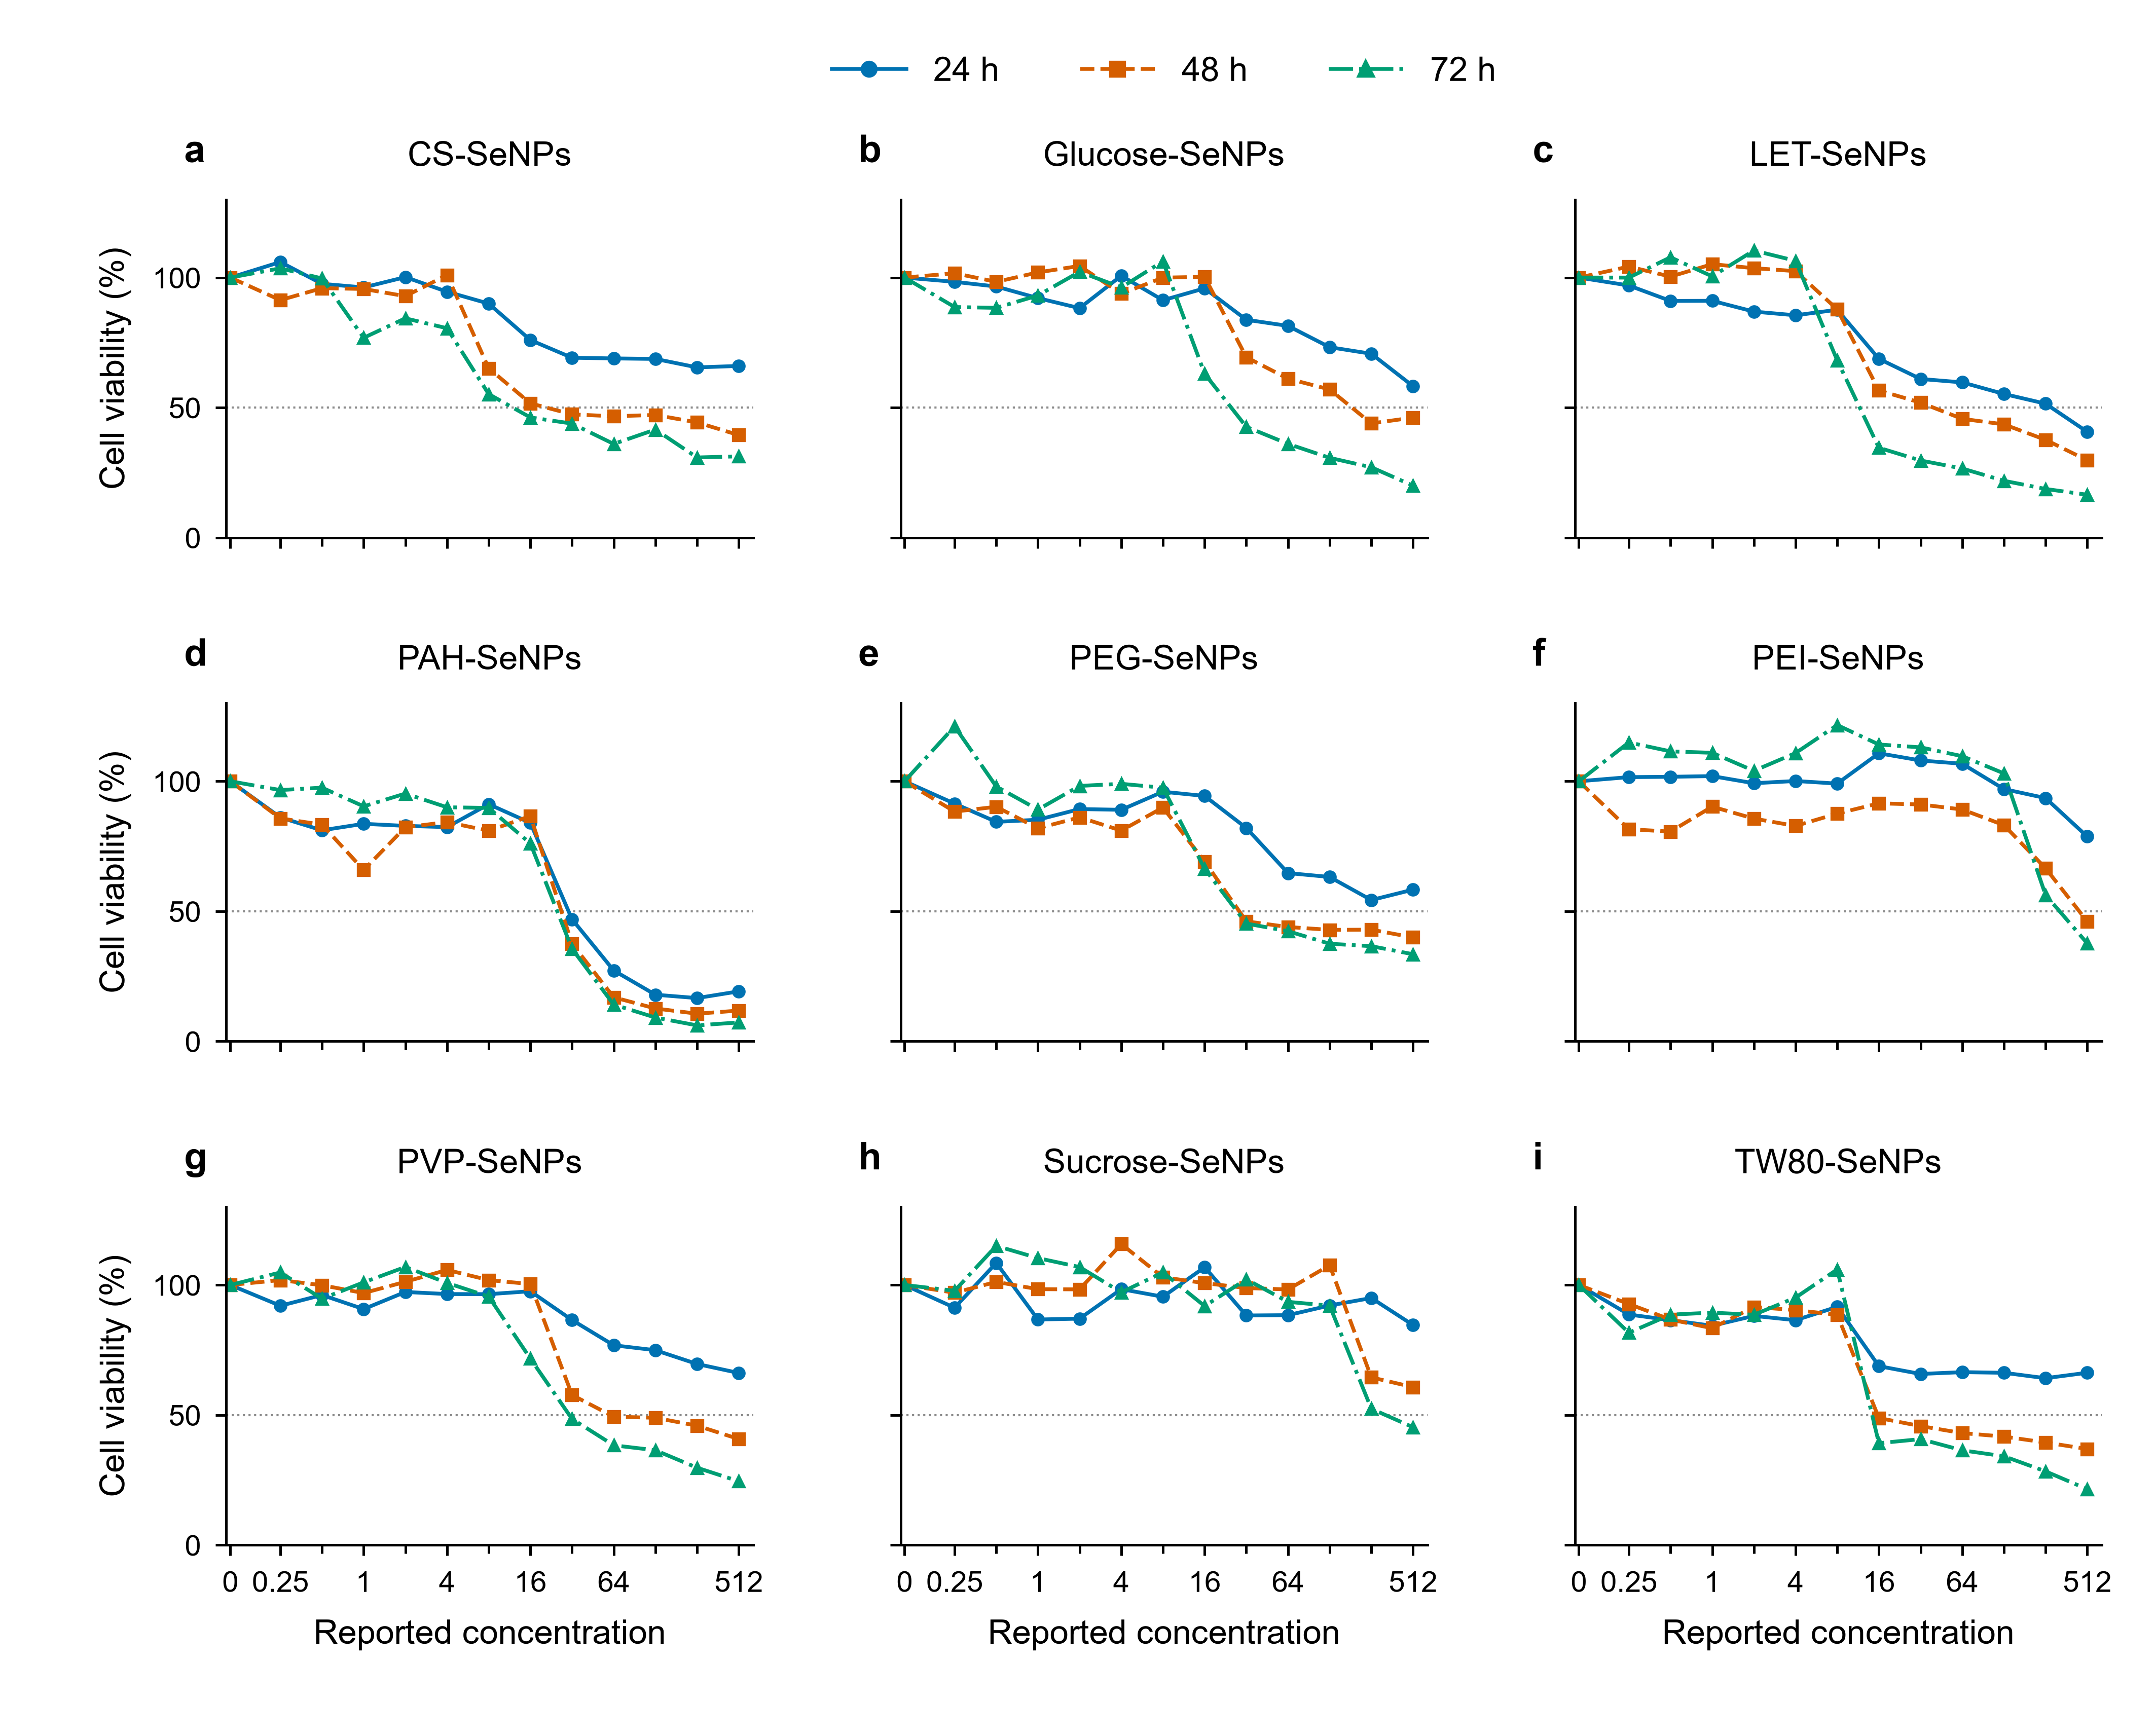
\includegraphics[width=\linewidth,height=0.70\textheight,keepaspectratio]{figures/huvec-dose-time.png}
\caption{9 种 SeNPs 在 HUVEC 中的剂量—时间报告曲线。a—i 依次为 CS、Glucose、LET、PAH、PEG、PEI、PVP、Sucrose 与 TW80。每个点为一个条件报告值，连线只连接报告点，虚线表示 50\% 存活率。浓度单位和计量基准待核实。}
\label{fig:huvec_dose_time}
\end{figure}

在报告浓度 512 下，以 9 种材料为分析单位，粒径与 24、48、72 h 存活率的 Spearman 系数分别为 0.200、0.383 和 0.267，Zeta 电位对应值为 0.050、\ensuremath{\mathord{-}}0.183 和 \ensuremath{\mathord{-}}0.050。这些描述性系数没有形成稳定的单变量关联证据，当前记录也不能区分粒径、电位、修饰化学及其他未测量因素的独立作用。依据冻结预测文件，已完成 351 个条件的预测—实测配对评价，并对 72 h、报告浓度 512 下的材料排序进行比较。

\subsection{冻结模型对新材料的存活率预测误差}

在351个材料—浓度—时间条件上，冻结模型预测与实验观测的总体 MAE 为 14.51 个存活率百分点，RMSE 为 20.11 个百分点，R\textsuperscript{2} 为 0.447，平均偏差为 +7.24 个百分点，表明模型在当前条件表中整体倾向于高估存活率（表~\ref{tab:huvec_external_performance}，图~\ref{fig:huvec_external_scatter}）。分时间点分析显示，24 h 的 MAE 和 RMSE 分别为 9.98 和 14.27 个百分点，48 h 分别为 13.99 和 18.86 个百分点，72 h 分别为 19.55 和 25.57 个百分点。预测误差随暴露时间延长而增大，提示模型未能充分捕捉较长暴露时间下的存活率下降。

在报告浓度 512 下，实验平均存活率在 24、48、72 h 分别为 59.81\%、39.07\% 和 26.38\%，模型预测均值则为 56.16\%、55.42\% 和 55.28\%。模型预测均值随时间变化较小，与实验观测的下降幅度不一致。上述结论限定于当前 9 种材料、HUVEC 体系和当前浓度映射，不能直接推广到其他细胞类型或材料。

\begin{table}[H]
\centering
\caption{冻结模型在 351 个 HUVEC 条件上的预测—实测误差。各条件不是独立实验重复。}
\label{tab:huvec_external_performance}
\small
\begin{tabular}{lrrrrr}
\toprule
时间 & n & MAE & RMSE & 预测均值 & 实测均值 \\
\midrule
24 h & 117 & 9.98 & 14.26 & 85.74 & 83.44 \\
48 h & 117 & 13.99 & 18.89 & 84.85 & 75.95 \\
72 h & 117 & 19.57 & 25.62 & 84.85 & 73.99 \\
总体 & 351 & 14.51 & 20.14 & 85.15 & 77.79 \\
\bottomrule
\end{tabular}

\end{table}

注：MAE、RMSE 的单位均为存活率百分点，均值单位为百分比。

\begin{figure}[H]
\centering
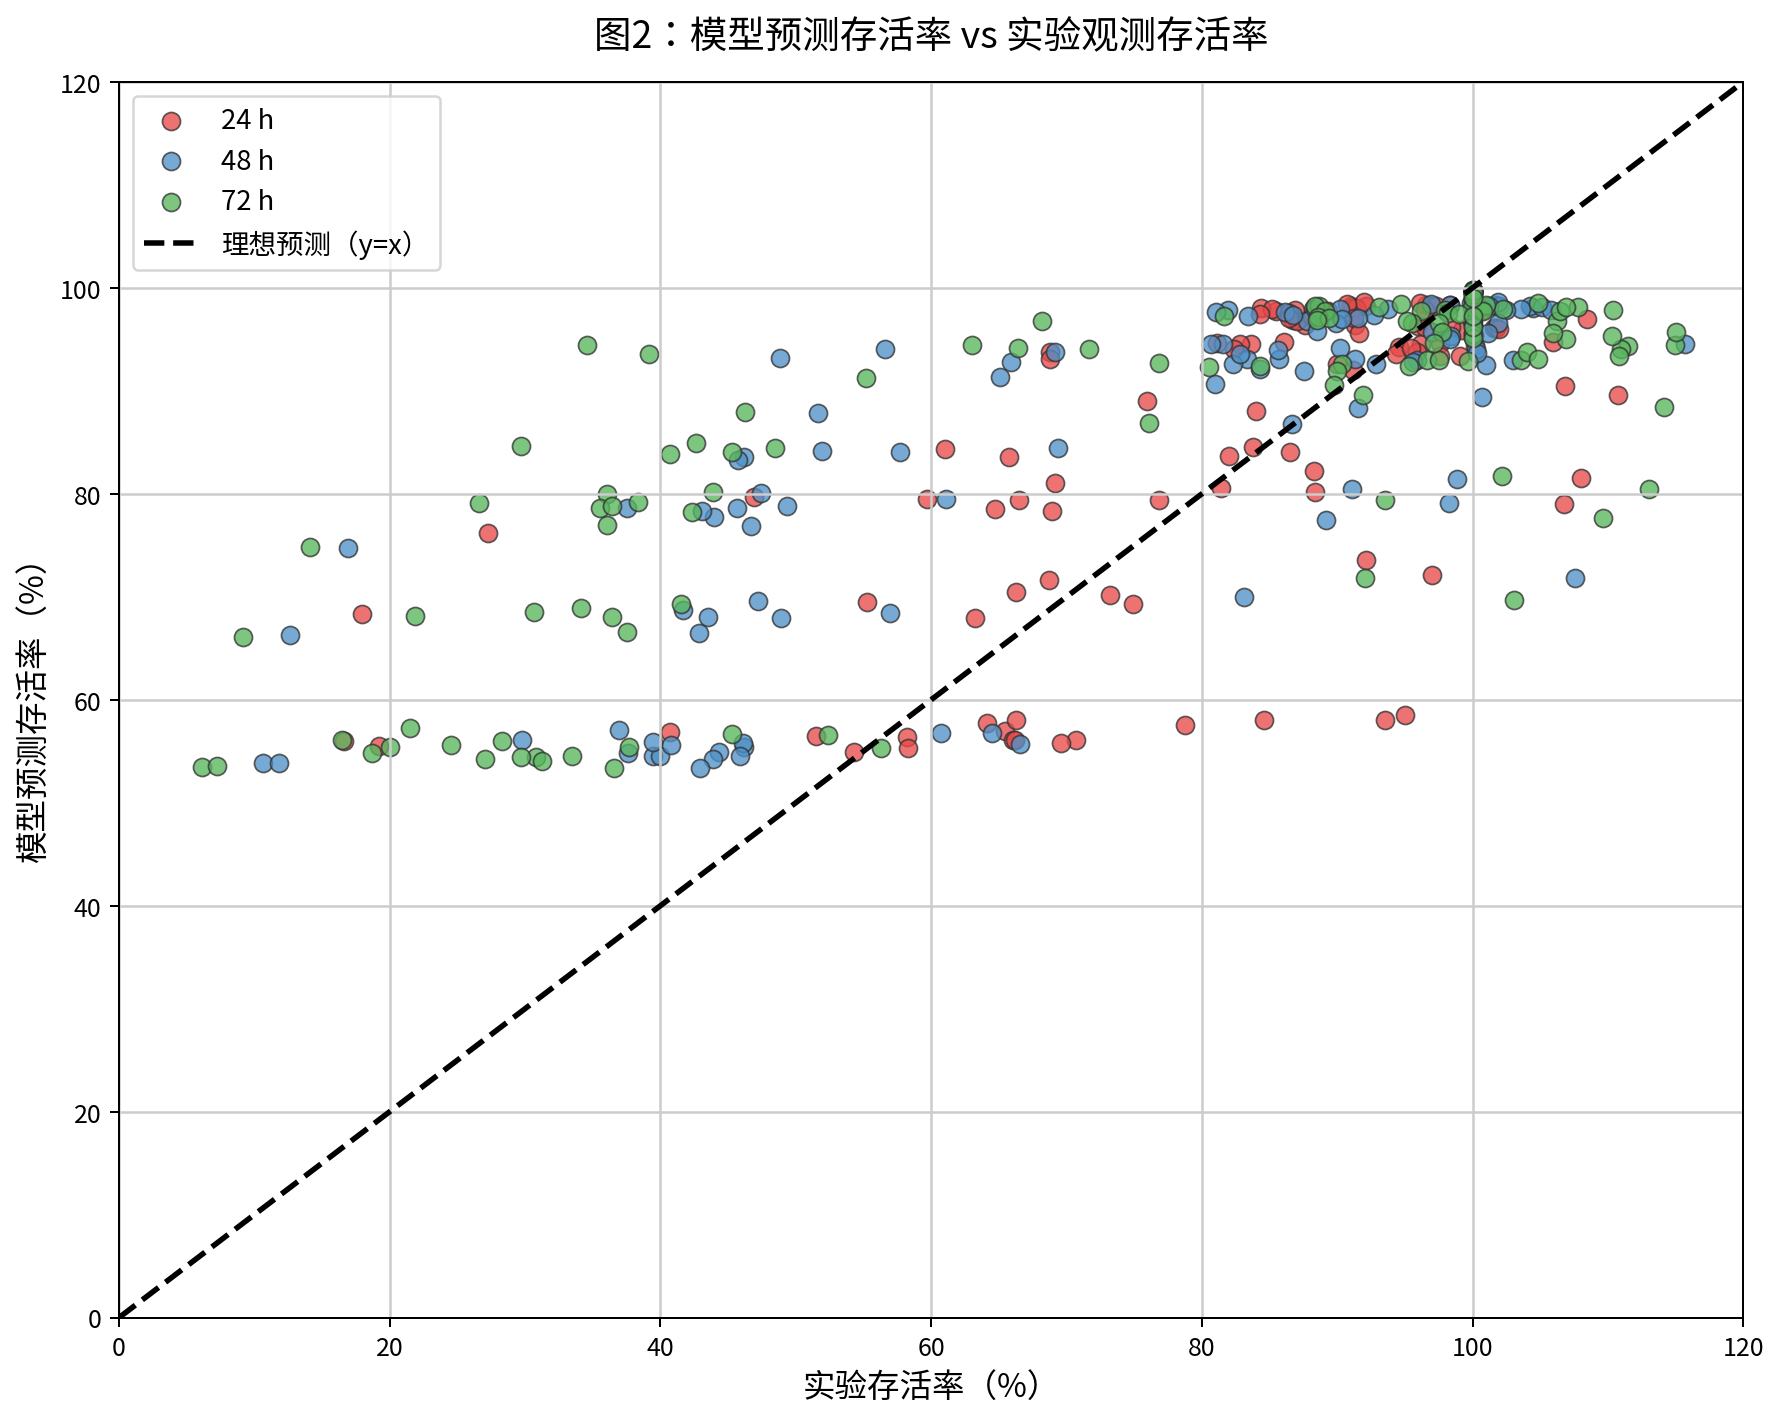
\includegraphics[width=\linewidth,height=0.70\textheight,keepaspectratio]{figures/scatter-viability.png}
\caption{冻结模型预测存活率与实验观测存活率的配对比较。虚线表示理想一致性线，颜色区分 24、48 和 72 h。}
\label{fig:huvec_external_scatter}
\end{figure}

\subsection{预测与实验毒性排序的一致性}

如图~\ref{fig:huvec_external_rank} 所示，在 HUVEC、72 h、报告浓度 512 的条件下，实验存活率从 PAH-SeNPs 的 7.26\% 到 Sucrose-SeNPs 的 45.30\%，跨度为 38.04 个百分点。相同条件下模型预测存活率集中在 53.54\% 至 56.69\% 之间，未能再现实验观测到的材料间差异。预测与实测排序的 Spearman 相关系数为 0.133，p = 0.732；Kendall \ensuremath{\tau} 为 0.111，p = 0.761。两项统计量均未显示可靠的排序一致性证据。由于分析单位为 9 种材料，结果应视为该指定条件下的描述性比较。

\begin{figure}[H]
\centering
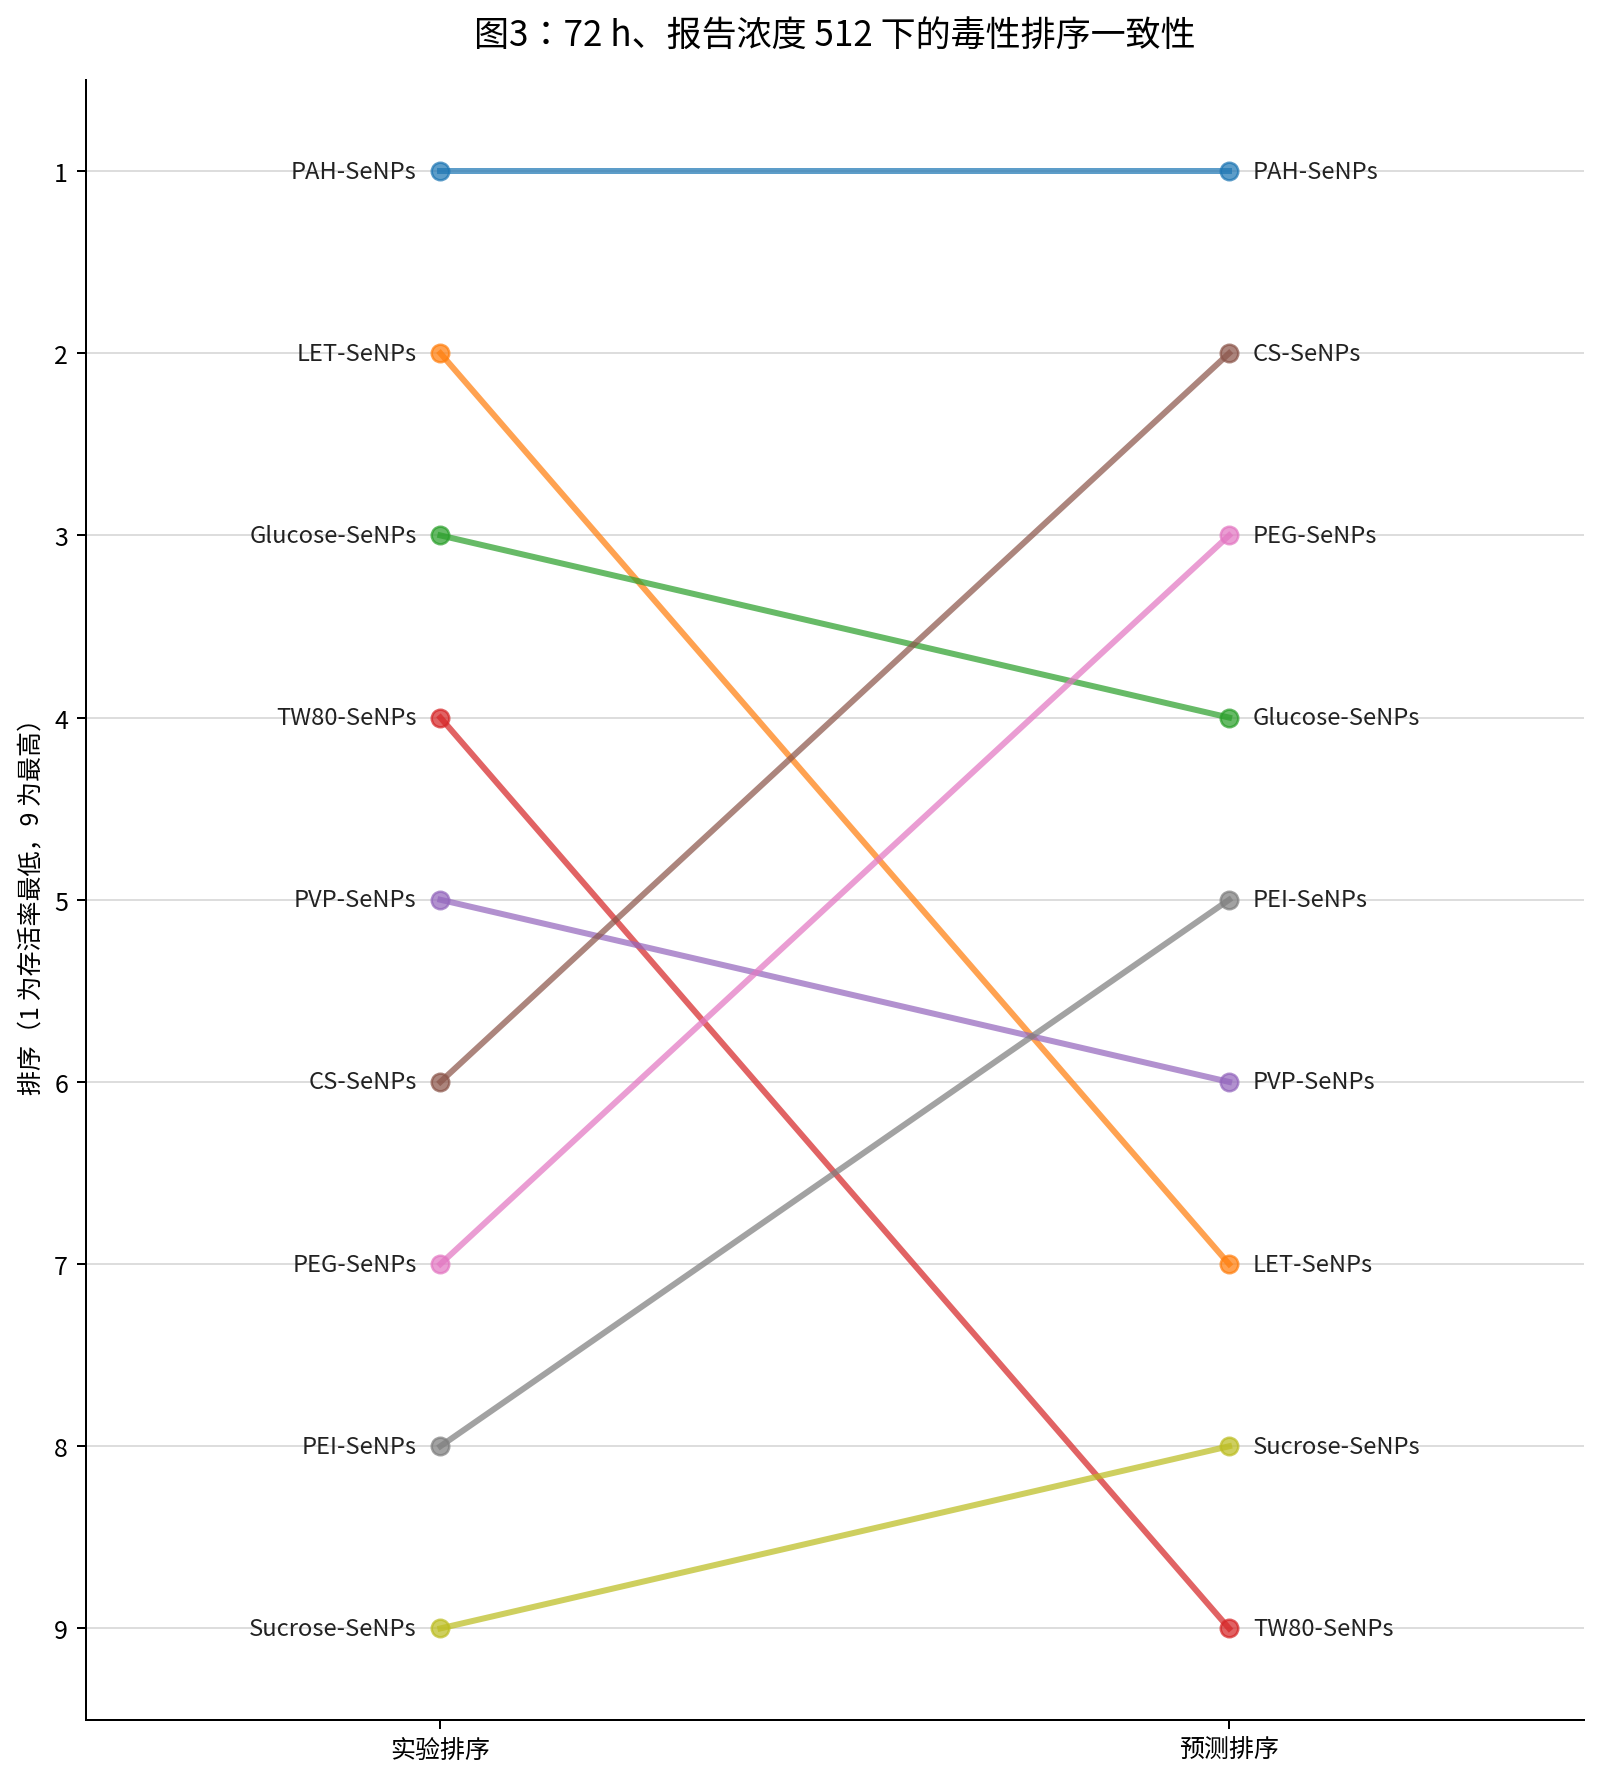
\includegraphics[width=\linewidth,height=0.70\textheight,keepaspectratio]{figures/rank-consistency.png}
\caption{72 h、报告浓度 512 下九种 SeNPs 的实验与预测毒性排序。排名 1 表示存活率最低、表观毒性最高，排名 9 表示存活率最高。}
\label{fig:huvec_external_rank}
\end{figure}

\subsection{粒径与 Zeta 电位的 SHAP 贡献}

图~\ref{fig:huvec_external_shap} 的 SHAP Summary Plot 展示了冻结随机森林对粒径组和 Zeta 相关特征组的预测贡献。图中各点代表一个材料—浓度—时间预测条件，横坐标为对预测存活率的有符号贡献，颜色表示相应描述符取值的高低。Zeta 组的贡献分布范围较宽，粒径组也呈现随条件变化的正负贡献。该结果说明模型在不同预测条件下使用这些特征的方式并不相同，但 SHAP 贡献反映的是模型内部的预测分配，不能解释为粒径或 Zeta 电位对细胞毒性的因果效应。

\begin{figure}[H]
\centering
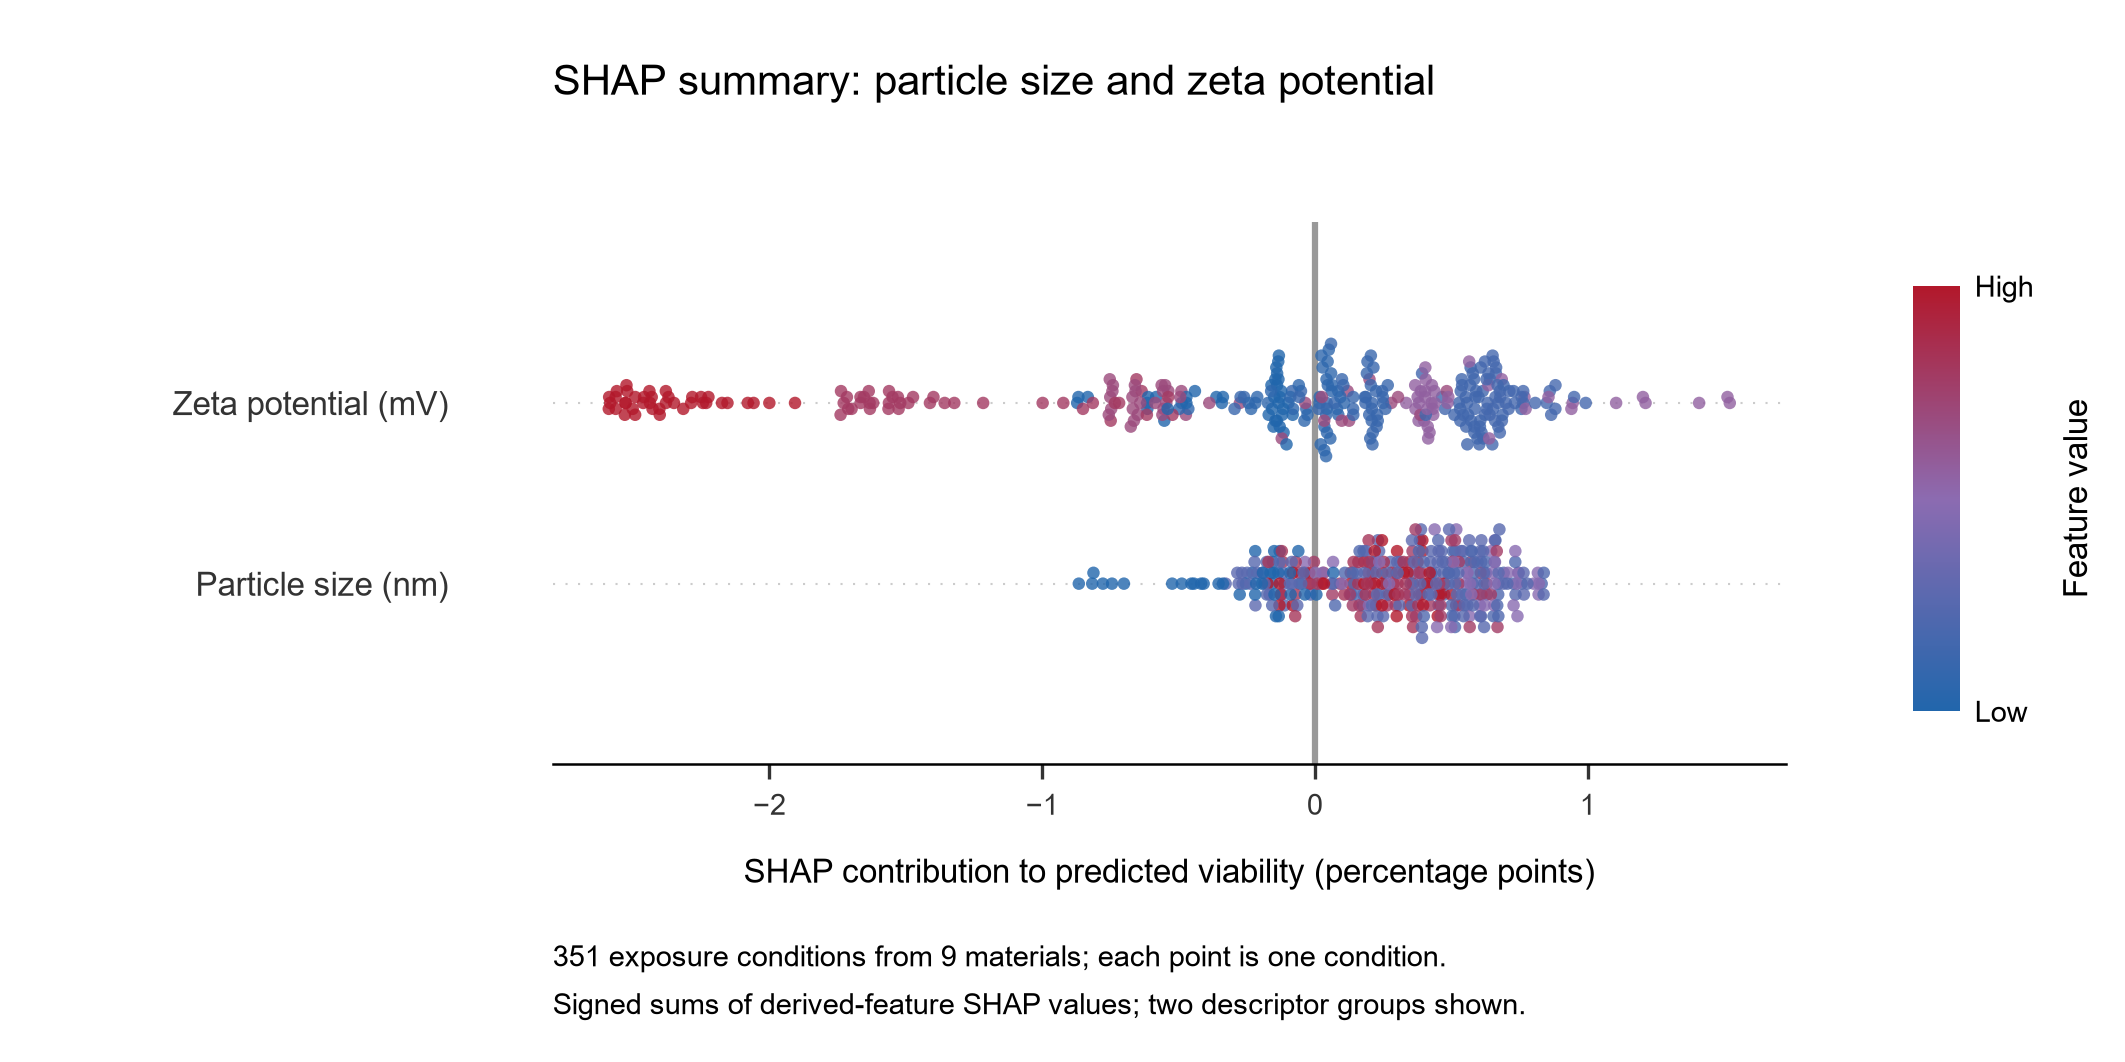
\includegraphics[width=\linewidth,height=0.70\textheight,keepaspectratio]{figures/shap-summary.png}
\caption{冻结随机森林模型中粒径与 Zeta 电位相关特征组的 SHAP Summary Plot。每个点为一个预测条件，不代表独立实验重复。}
\label{fig:huvec_external_shap}
\end{figure}

\subsection{预测问题的界定与材料信息的实际增量}

本研究把历史模型评价和新增实验观测置于同一研究问题下，同时保留两者不同的证据任务。历史分组结果显示，当前基础输入对跨文献存活率的预测仍有较大误差，更多化学字段、显式剂量—时间交互与固定预算迁移没有稳定降低误差；新增实验则提供了真实材料在 HUVEC 中的响应曲线，展示了时间变化与条件相关的材料差异。两部分共同说明，预测性能和实验响应结构需要各自获得直接证据，方向一致的实验趋势不足以替代逐样本预测评价。

化学增强的阴性结果限定于当前字段质量、样本组成与模型配置，并不说明材料化学性质在毒性形成中没有作用。历史数据的 Zeta 电位缺失率为 42.40\%，修饰物类别和分子量没有完整字段，晶体信息编码又只反映是否报告晶体学信息，这些条件限制了模型对材料差异的识别。表征方法、报告习惯和研究环境还可能共同影响输入值，新增字段是否具有生物学意义，与其能否在当前归档数据中提供稳定预测增量，属于需要分开讨论的问题。

同样，迁移对照尚未建立稳定收益，可能与不同材料体系的响应分布、共同特征的覆盖以及当前树模型迁移接口有关。RF 的新增树训练保留原有通用树，XGBoost 的续训依赖已学习的通用结构，本研究没有检验其他迁移方法，不能将结果推广为迁移学习对 SeNPs 普遍无效。对于现阶段的材料筛选，更合适的工作是明确模型可接受的输入、记录外部测试条件，并检验预测误差，而不是根据通用基准指标直接判断新材料预测精度。

\subsection{与既有计算研究的关系}

Gul 等的跨材料属性分析与 Masarkar 等的预测研究，为组织纳米材料理化性质、细胞背景和暴露条件提供了基础 \cite{gul2021association,masarkar2024}。本研究进一步关注这些信息在 SeNPs 文献分组评价下的增量，以及新增实验如何与历史建模衔接。由于数据纳入、特征定义、模型选择与验证划分均不同，本研究不以跨论文的单个 $R^2$ 或 MAE 数值宣称性能优于既有工作，早期深度模型指标作为历史探索保留，不纳入后续分组评价的统一模型排名。

嵌套评价使内层选择与外层报告分离，对有限样本下模型选择偏差的控制与已有方法学研究一致 \cite{cawley2010selection}。不过，文献分组验证只检验对未参与训练的文献组的表现，不能自动代表对未知配方、未知修饰物或不同实验室的泛化。旧历史复现还混合了随机交叉验证误差、全量拟合 $R^2$ 和不同预处理设置，当前结果不构成只改变划分方式的受控对照，因此性能差异不能全部归因于随机划分造成的泄漏，方法与数据口径的变化也需要保留在解释中。

\subsection{实验观测的意义与机制解释范围}

HUVEC 数据把研究从历史文献预测扩展到真实材料的剂量—时间观测，最高测试浓度下的时间变化与有限 IC50 估计数量的增加共同表明，评价时间会影响材料差异的呈现方式。对照已有SeNPs 细胞研究，这些结果支持将材料修饰和暴露条件一起纳入实验比较 \cite{wang2020prooxidation,lunkov2023chitosan}，但当前单一细胞模型不能提供正常与肿瘤细胞选择性、跨细胞普适性或体内安全性的证据。

材料的高浓度排序与表观 IC50 排序并不一致，反映了固定浓度残余存活率与跨越 50\% 阈值所处位置的不同。表观 IC50 仅由两个相邻报告点插值，浓度间距、局部波动和检测读数都可能影响估计，尚不能用于给出精细的材料优劣判断。对没有跨越阈值的曲线保留 > 512 状态，也避免了在测试范围外强行拟合一个看似完整的数值。

粒径、电位和修饰信息在不同材料之间同时变化，每种材料又仅有一组描述符报告值，因此弱秩相关既不能证明这些性质无作用，也不能将某种材料的低存活率归因于单个描述符。大于 100\%的报告值同样需要谨慎解释，当前缺少原始孔读数、空白扣除及检测干扰信息，不能据此判定真实增殖促进或特定毒性机制。核对这些实验信息后，才能进一步评估剂量曲线的波动与材料相关的检测影响。

\subsection{外部预测评价仍需完成的环节}

按材料、报告浓度、时间及浓度单位匹配后获得 351 对预测—实测值，因而本研究可以报告当前条件表上的 MAE、RMSE、平均偏差及预测—实测排序一致性。每个条件只有一个归档报告值，不能据此估计独立实验重复间的变异。实测 IC50 不能作为新材料初筛模型的输入。
